%versi 2 (8-10-2016)

\lstdefinelanguage{plaintext}{
  sensitive=false,
  comment=[l]{//},
  morecomment=[s]{/*}{*/},
  identifierstyle=\color{black},
  morestring=[b]',
  morestring=[b]"
}

\lstset
{ 
    language=plaintext,
    basicstyle=\footnotesize,
    numbers=left,
    stepnumber=1,
    showstringspaces=false,
    tabsize=1,
    breaklines=true,
    breakatwhitespace=false,
    frame=leftline
}



\chapter{Landasan Teori}
\label{chap:teori}

Pada bab ini dibahas dasar teori yang mendukung skripsi ini. Dasar teori yang dibahas yaitu Version Control Systems, Git, JGit, Selenium WebDriver, dan Apache Commons CLI.

\section{Version Control Systems}
\label{sec:Version Control Systems}
\textit{Version Control Systems} adalah sistem yang merekam perubahan pada \textit{file} atau sekumpulan \textit{file} dari waktu ke waktu.\textit{Version Control Systems} biasanya digunakan  untuk merekam file yang berisi \textit{source code program}, tetapi pada kenyataannya \textit{Version Control Systems} dapat merekam semua jenis file dalam komputer. Terdapat tiga jenis \textit{Version Control Systems}, yaitu: \textit{Local Version Control Systems}, \textit{Centralized Version Control Systems}, dan \textit{Distributed Version Control Systems}. 

\subsection{Local Version Control Systems}
\label{subsec:lvcs}
Metode pengendalian versi yang biasa digunakan adalah dengan cara menyalin sekumpulan \textit{file} ke direktori lain. Namun cara tersebut rentan terhadap \textit{error}.
Misalnya, terdapat direktori A dan B, pengguna ingin mengubah \textit{file} yang terdapat pada direktori B, tetapi pengguna lupa kalau dia sedang berada di direktori A, maka pengguna mengubah \textit{file} pada direktori yang salah. Untuk mengatasi masalah tersebut, dikembangkanlah \textit{Local Version Control Systems}. 

\begin{figure}[H]
	\centering
		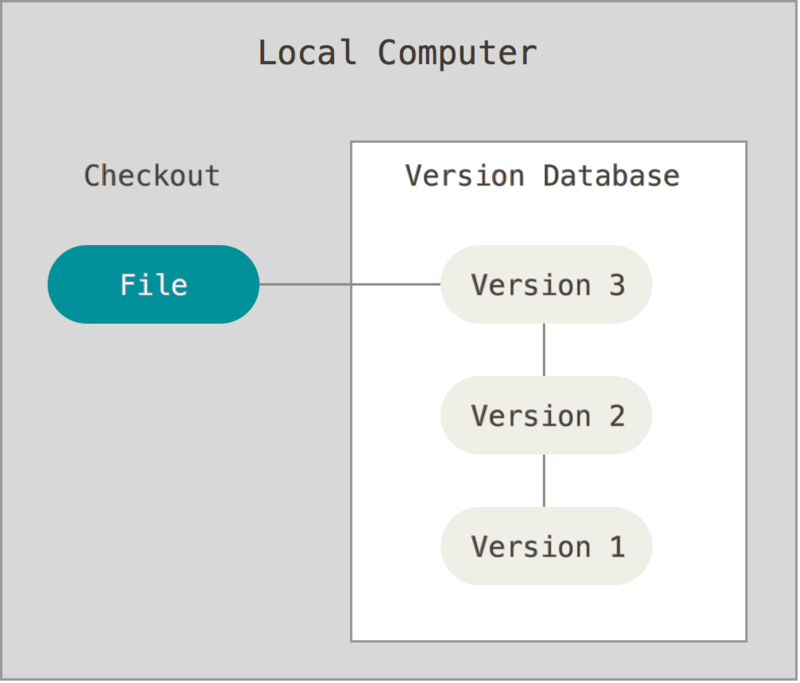
\includegraphics[scale=0.25]{Gambar/localvcs.png}
	\caption{Local version control\cite{chacon2014pro}.}
	\label{fig:localvcs}
\end{figure}

Gambar \ref{fig:localvcs} merupakan struktur dari \textit{Local Version Control Systems}. \textit{Database local Version Control Systems} ini tersimpan pada direktori lokal di komputer. \textit{Database} ini menyimpan perubahan \textit{file} ke dalam beberapa versi.  
 
\subsection{Centralized Version Control Systems}
\label{subsec:cvcs}
\begin{figure}[H]
	\centering
		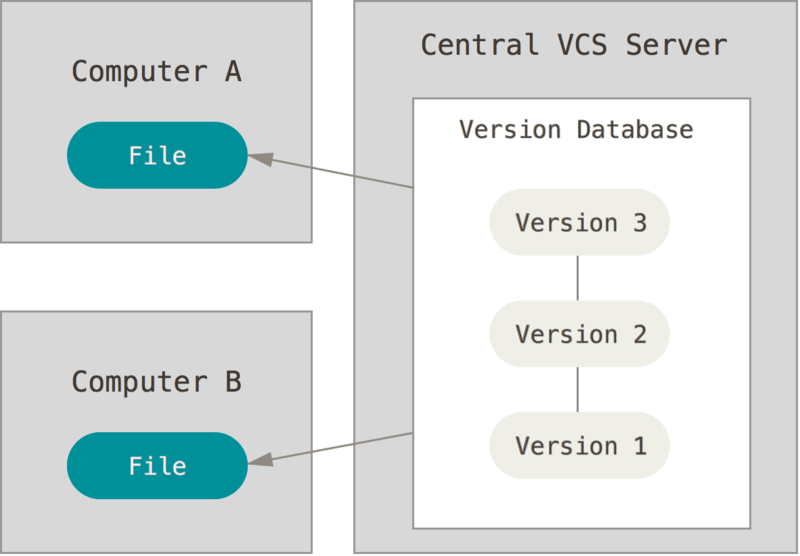
\includegraphics[scale=0.25]{Gambar/centralizedvcs.png}
	\caption{Centralized version control\cite{chacon2014pro}.}
	\label{fig:cvcs}
\end{figure}

\textit{Local Version Control} hanya menyimpan \textit{file} pada satu komputer saja. Muncul masalah baru ketika \textit{user} ingin berkolaborasi dengan \textit{user} lain. Untuk mengatasi masalah ini dikembangkan \textit{Centralized version control}. Gambar \ref{fig:cvcs} merupakan struktur dari \textit{Centralized Version Control Systems}. Dalam \textit{Centralized Control Version Systems} terdapat sebuah \textit{server} yang menyimpan setiap versi \textit{file}, dan klien yang dapat melakukan \textit{checkout} \textit{file}.

Sistem \textit{Centralized Version Control Systems} memiliki beberapa kelebihan. Setiap \textit{user}  dapat mengetahui pekerjaan yang dilakukan oleh \textit{user} lain. Administrator dapat lebih mudah mengontrol \textit{database} \textit{Centralized Version Control Systems} dibandingkan dengan \textit{database} \textit{Local Version Control Systems} dari setiap klien.      

Sistem \textit{Centralized Version Control Systems} memiliki kelemahan. Jika \textit{server} pusat \textit{Centralized Version Control Systems} mati, maka perubahan pada \textit{file} tidak bisa disimpan. Klien juga tidak dapat melakukan kolaborasi dengan klien lain. Jika \textit{harddisk} pada server rusak, maka semua versi \textit{file} akan hilang.  

\subsection{Distributed Version Control Systems}
\label{subsec:dvcs}
\begin{figure}[H]
	\centering
		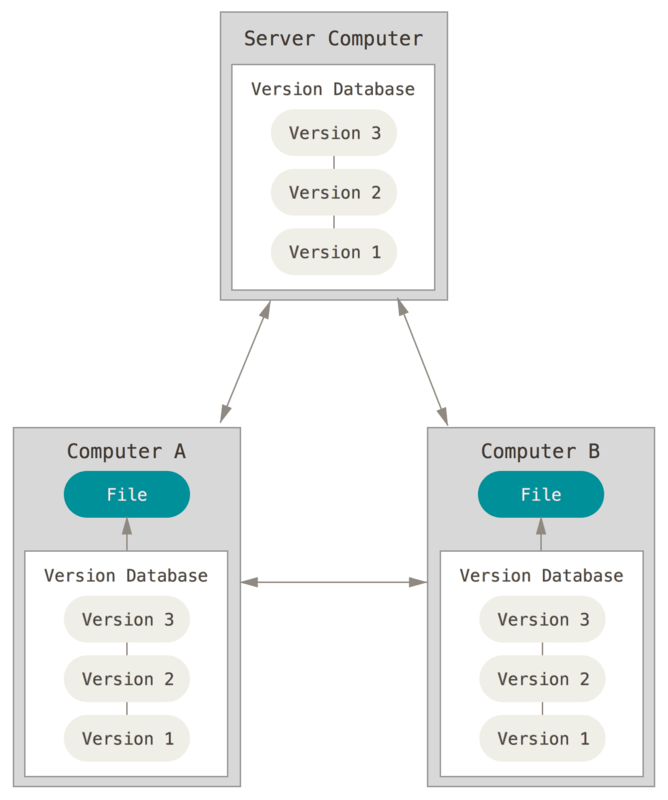
\includegraphics[scale=0.5]{Gambar/dvcs.png}
	\caption{Distributed version control\cite{chacon2014pro}.}
	\label{fig:dvcs}
\end{figure}
Gambar \ref{fig:dvcs} merupakan struktur dari \textit{Distributed Version Control Systems}. Dalam sebuah DVCS (seperti Git, Mercurial, Bazaar atau Darcs), klien tidak hanya melakukan \textit{checkout} untuk \textit{snapshot} terakhir setiap \textit{file}, namun klien juga memiliki salinan dari repositori tersebut. Dengan kata lain setiap klien memiliki \textit{version database local} pada komputernya. Jika server pusat mati, klien masih bisa melakukan kolaborasi dan klien manapun dapat mengirimkan kembali salinan repositori ke \textit{server}.


\section{Git}
\label{sec:git} 
%Git merupakan perangkat lunak \textit{Version Control Systems}. 
Pada subbab ini, dijelaskan mengenai cara kerja Git, Git \textit{checkout}, dan operasi-operasi dasar pada Git. Subbab ini mengacu pada \cite{chacon2014pro}.   

%\subsection{Version Control Systems}
%\label{subsec:vcs}
%\textit{Version Control Systems} adalah sistem yang merekam perubahan pada \textit{file} atau sekumpulan \textit{file} dari waktu ke waktu.\textit{Version Control Systems} biasanya digunakan  untuk merekam file yang berisi \textit{source code program}, tetapi pada kenyataannya \textit{Version Control Systems} dapat merekam semua jenis file dalam komputer. Terdapat tiga jenis \textit{Version Control Systems}, yaitu: \textit{Local Version Control Systems}, \textit{Centralized Version Control Systems}, dan \textit{Distributed Version Control Systems}.

%\subsubsection{Local Version Control Systems}
%Metode pengendalian versi yang biasa digunakan adalah dengan cara menyalin sekumpulan \textit{file} ke direktori lain. Namun cara tersebut rentan terhadap \textit{error}.
%Misalnya, terdapat direktori A dan B, pengguna ingin mengubah \textit{file} yang terdapat pada direktori B, tetapi pengguna lupa kalau dia sedang berada di direktori A, maka pengguna mengubah \textit{file} pada direktori yang salah. Untuk mengatasi masalah tersebut, dikembangkanlah \textit{Local Version Control Systems}. 

%\begin{figure}[H]
%	\centering
%		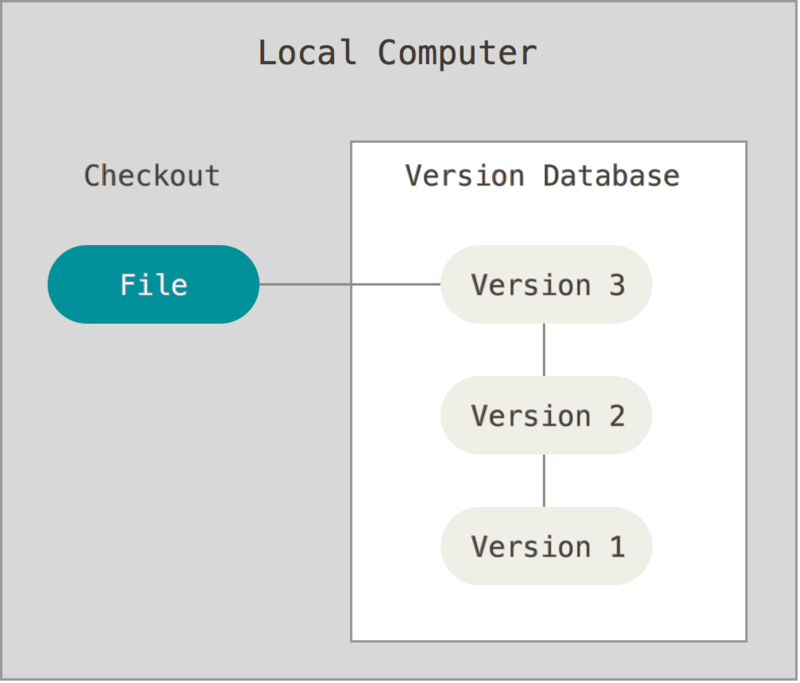
\includegraphics[scale=0.25]{Gambar/localvcs.png}
%	\caption{Local version control\cite{chacon2014pro}.}
%	\label{fig:localvcs}
%\end{figure}

%Gambar \ref{fig:localvcs} merupakan struktur dari \textit{Local Version Control Systems}. \textit{Database local Version Control Systems} ini tersimpan pada direktori lokal di komputer. \textit{Database} ini menyimpan perubahan \textit{file} ke dalam beberapa versi.  
 
%\subsubsection{Centralized Version Control Systems}
%\begin{figure}[H]
%	\centering
%		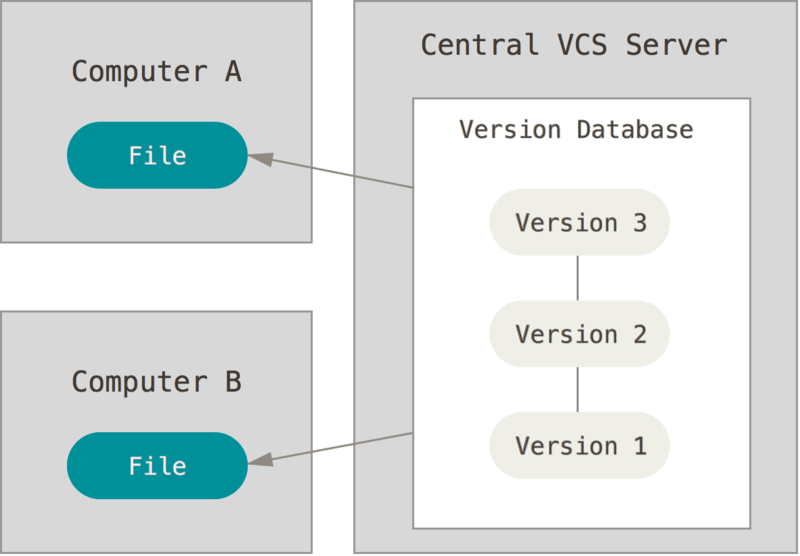
\includegraphics[scale=0.25]{Gambar/centralizedvcs.png}
%	\caption{Centralized version control\cite{chacon2014pro}.}
%	\label{fig:cvcs}
%\end{figure}

%\textit{Local Version Control} hanya menyimpan \textit{file} pada satu komputer saja. Muncul masalah baru ketika \textit{user} ingin berkolaborasi dengan \textit{user} lain. Untuk mengatasi masalah ini dikembangkan \textit{Centralized version control}. Gambar \ref{fig:cvcs} merupakan struktur dari \textit{Centralized Version Control Systems}. Dalam \textit{Centralized Control Version Systems} terdapat sebuah \textit{server} yang menyimpan setiap versi \textit{file}, dan klien yang dapat melakukan \textit{checkout} \textit{file}.

%Sistem \textit{Centralized Version Control Systems} memiliki beberapa kelebihan. Setiap \textit{user}  dapat mengetahui pekerjaan yang dilakukan oleh \textit{user} lain. Administrator dapat lebih mudah mengontrol \textit{database} \textit{Centralized Version Control Systems} dibandingkan dengan \textit{database} \textit{Local Version Control Systems} dari setiap klien.      

%Sistem \textit{Centralized Version Control Systems} memiliki kelemahan. Jika \textit{server} pusat \textit{Centralized Version Control Systems} mati, maka perubahan pada \textit{file} tidak bisa disimpan. Klien juga tidak dapat melakukan kolaborasi dengan klien lain. Jika \textit{harddisk} pada server rusak, maka semua versi \textit{file} akan hilang.  

%\subsubsection{Distributed Version Control Systems}
%\begin{figure}[H]
%		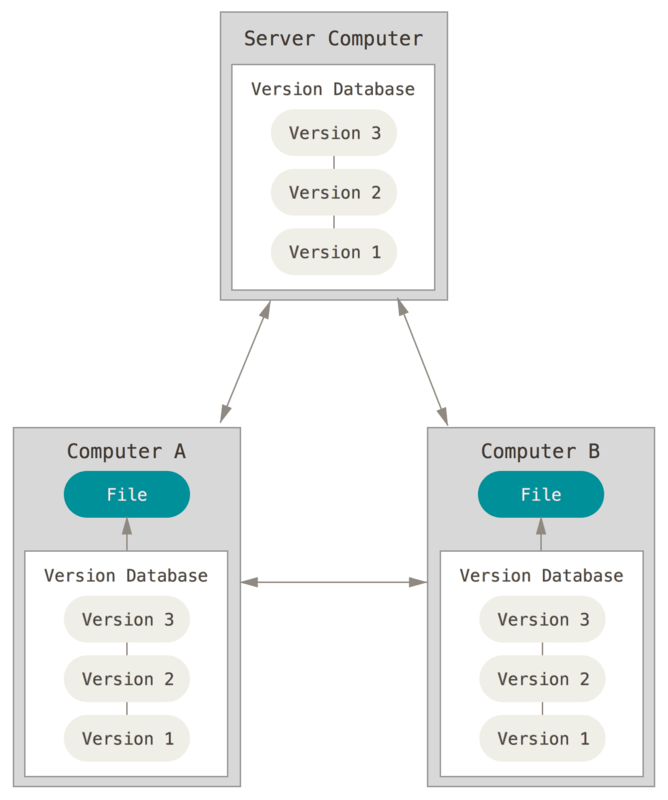
\includegraphics[scale=0.5]{Gambar/dvcs.png}
	%\caption{Distributed version control\cite{chacon2014pro}.}
%	\label{fig:dvcs}
%\end{figure}
%Gambar \ref{fig:dvcs} merupakan struktur dari \textit{Distributed Version Control Systems}. Dalam sebuah DVCS (seperti Git, Mercurial, Bazaar atau Darcs), klien tidak hanya melakukan \textit{checkout} untuk \textit{snapshot} terakhir setiap \textit{file}, namun klien juga memiliki salinan dari repositori tersebut. Dengan kata lain setiap klien memiliki \textit{version database local} pada komputernya. Jika server pusat mati, klien masih bisa melakukan kolaborasi dan klien manapun dapat mengirimkan kembali salinan repositori ke \textit{server}.

\subsection{Cara Kerja Git}
\label{subsec:cara_kerja_git}
Salah satu perbedaan antara Git dengan VCS lainnya adalah dalam cara Git memperlakukan datanya. Kebanyakan sistem \textit{Version Control Systems} lain menyimpan informasi sebagai daftar perubahan \textit{file}. Pada Gambar \ref{fig:deltas}, terdapat tiga \textit{file}.\textit{Version Control Systems} menyimpan \textit{file} A, B, dan C pada versi pertama saja. Untuk versi kedua dan seterusnya yang disimpan adalah perubahan pada setiap \textit{file}. Sistem ini disebut juga sebagai \textit{delta-based Version Control Systems}. 
\begin{figure}[H]
	\centering
		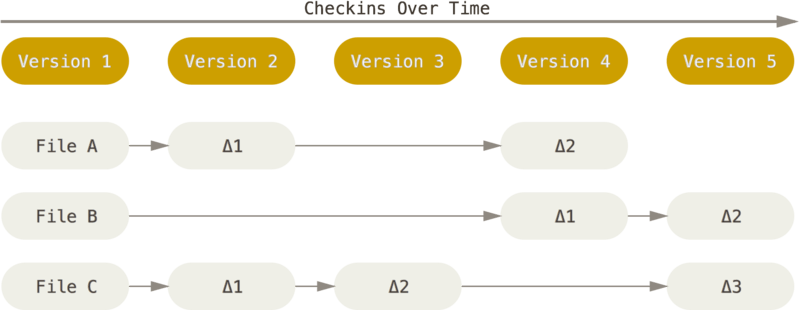
\includegraphics[scale=0.5]{Gambar/deltas.png}
	\caption{Menyimpan data sebagai \textit{snapshots} dari \textit{project}\cite{chacon2014pro}.}
	\label{fig:deltas}
\end{figure}


Berbeda dengan \textit{Version Control Systems} lainnya, Git memperlakukan datanya sebagai sebuah kumpulan \textit{snapshot} dari sebuah miniatur \textit{file system}. Setiap kali dilakukan \textit{commit}, Git merekam \textit{state} dari sekumpulan \textit{file} dan menyimpannya sebagai \textit{snapshot}. Gambar \ref{fig:snapshots}, menunjukkan \textit{snapshots} dari \textit{file} A, B, dan C. Pada versi kedua, \textit{file} B tidak mengalami perubahan, sehingga yang disimpan adalah \textit{reference} dari \textit{file} B pada versi sebelumnya.
\begin{figure}[H]
	\centering
		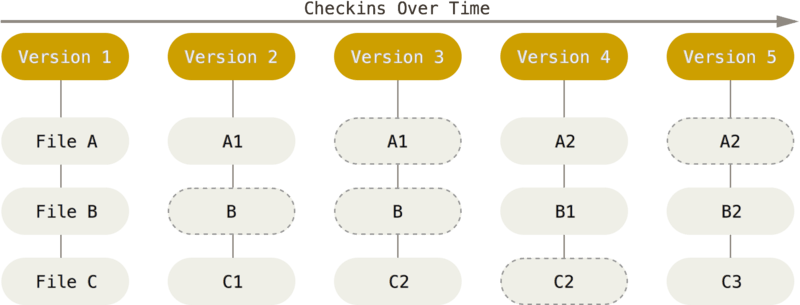
\includegraphics[scale=0.5]{Gambar/snapshots.png}
	\caption{Menyimpan data sebagai perubahan terhadap versi dasar dari setiap \textit{file}\cite{chacon2014pro}.}
	\label{fig:snapshots}
\end{figure}

\subsubsection{State pada Git}
Terdapat tiga \textit{state} pada Git yaitu \textit{committed}, \textit{modified}, and \textit{staged}. \textit{Committed} adalah \textit{state} dimana data sudah disimpan di \textit{local database}. \textit{Modified} adalah \textit{state} dimana terdapat perubahan pada \textit{file}, namun \textit{file} tersebut belum di \textit{commit} ke \textit{database}. \textit{Staged} adalah \textit{state} dimana \textit{file} telah ditandai untuk kemudian dilakukan \textit{commit}.

Terdapat tiga bagian utama dari sebuah \textit{project} Git yaitu direktori Git, \textit{working directory}, dan \textit{staging area}. Direktori Git merupakan tempat dimana Git menyimpan \textit{metadata} dan \textit{object database} dari \textit{project}. \textit{Working directory} adalah suatu \textit{snapshot} dari \textit{project}. Sekumpulan \textit{file} ini diambil dari \textit{database} di direktori Git dan ditempatkan pada \textit{disk} untuk digunakan dan dimodifikasi. \textit{Staging} area adalah suatu \textit{file} dimana \textit{file} ini menyimpan daftar \textit{file} yang telah ditandai untuk kemudian dilakukan \textit{commit}. \textit{File staging area} terdapat pada direktori Git. Untuk lebih jelasnya dapat dilihat Gambar \ref{fig:git_state}.

Alur kerja dari Git adalah sebagai berikut:
\begin{enumerate}
\item Melakukan modifikasi pada \textit{file}.
\item Menandai perubahan pada \textit{file} dan memindahkannya ke \textit{staging area}.
\item Mengambil \textit{file} dari \textit{staging area} dan menyimpan \textit{snapshot} ke direktori Git. Proses ini disebut dengan \textit{commit}.
\end{enumerate}  

\begin{figure}[H]
	\centering
		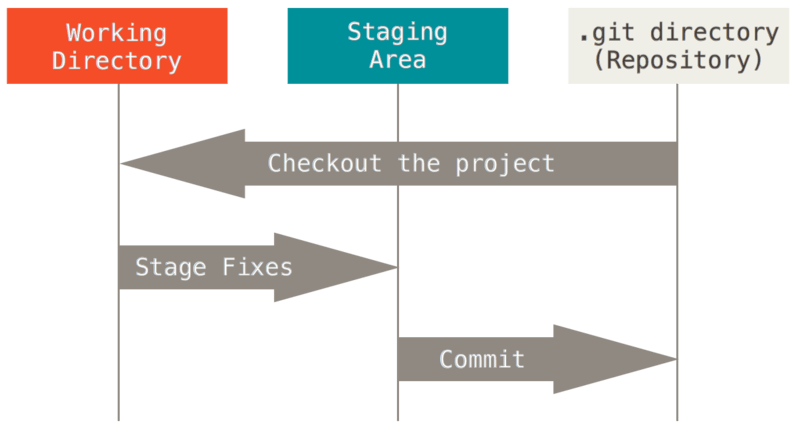
\includegraphics[scale=0.5]{Gambar/git_state.png}
	\caption{ \textit{Working directory}, \textit{Staging area}, dan Git direktori\cite{chacon2014pro}.}
	\label{fig:git_state}
\end{figure}

\subsubsection{Commit}
Commit merupakan sebuah \textit{snapshot} dari suatu \textit{file} atau direktori. Dengan kata lain yang disimpan oleh Git adalah \textit{state} dari \textit{file} atau direktori pada suatu waktu. \textit{File} disimpan oleh Git dalam bentuk \textit{blob}, sedangkan direktori disimpan dalam bentuk \textit{tree}. \textit{Commit}, \textit{blob}, dan \textit{tree} merupakan Git Object. Setiap Git Object memiliki ID berupa SHA-1 \textit{hash value} dengan panjang empat puluh karakter heksadesimal. 


%\textit{Commit} menggambarkan \textit{state} dari \textit{working directory}. Gambar \ref{fig:snapshots} menunjukkan terdapat tiga \textit{file} pada \textit{version} 4. Dimana terdapat \textit{file} A1, B1, dan C1 pada \textit{working directory}. \textit{File} A1, B1, dan C2  merupakan \textit{state} \textit{file} A, B, dan C pada \textit{version} 4. 

%Git melakukan \textit{checksum} pada \textit{commit} sebelum menyimpannya ke direktori Git. Mekanisme yang digunakan untuk melakukan \textit{check-summed} disebut dengan \textit{SHA-1 hash}. \textit{SHA-1 hash} terdiri dari empat puluh karakter heksadesimal(0-9 a-f). Nilai dari \textit{SHA-1 hash} dihitung berdasarkan isi dari\textit{working directory} atau struktur direktori Git.


\begin{lstlisting}[caption={Contoh \textit{commit history} dalam pengembangan perangkat lunak},label={lst:git_histori},language=plaintext]
commit 89000be7ce7d16f006813cddefb4ec6d70d15ed6 (HEAD -> master, origin/master, origin/HEAD)
Author: Hizkia Steven <xvii.hs@gmail.com>
Date:   Fri Jan 12 12:25:30 2018 +0700

    Update new company address

commit 6a085c1c37949e6308cfe06a117302e528388e54
Author: Hizkia Steven <xvii.hs@gmail.com>
Date:   Tue Dec 12 14:38:38 2017 +0700

    Update company address

commit 9f041ef239bfe236ab4d679ad698d773a8ba6f56
Author: TommyAdhityaThe <toms.warior@gmail.com>
Date:   Mon May 15 10:40:16 2017 +0700

    set insta url to https://www.instagram.com/piktorastudio/

commit 38711f0cc8f487aac62babac10c1185f5ee14d33
Author: Tommy Adhitya The <toms.warior@gmail.com>
Date:   Mon Apr 17 15:15:03 2017 +0700

    fix bug ugly display when projects too high
    
\end{lstlisting}

Listing \ref{lst:git_histori} menunjukkan sebagian \textit{commit history} pada \textit{branch} master. Baris pertama menunjukkan \textit{commit} ID berupa \textit{SHA-1 hash value}, dengan panjang empat puluh karakter heksadesimal. Baris kedua menunjukkan orang yang melakukan \textit{commit} dan alamat emailnya. Baris ketiga menunjukkan waktu \textit{commit}. Baris terakhir berisi deskripsi dari \textit{commit} tersebut.

HEAD dan \textit{master} pada Listing \ref{lst:git_histori}, disebut juga dengan Git Ref / Reference. Ref merupakan suatu variabel yang menyimpan ID (SHA-1 hash value) dari suatu Git Object. Pada Listing \ref{lst:git_histori}, Ref \textit{master} menyimpan ID dari \textit{commit} yang isinya adalah 89000be7ce7d16f006813cddefb4ec6d70d15ed6. Ref HEAD tidak secara langsung menyimpan ID dari \textit{commit}, melainkan \textit{pointer} ke Ref \textit{master}. Ref yang menyimpan \textit{pointer} ke Ref lain disebut juga dengan \textit{symbolic Ref}. 

Ref origin/master merupakan Ref \textit{master} yang berada pada \textit{remote repository}. 
Ref origin/HEAD merupakan ref HEAD yang berada pada \textit{remote repository}. \textit{Remote repository} merupakan repositori yang disimpan pada suatu \textit{server}, misalnya \textit{server} GitHub. 

\subsection{Operasi Dasar pada Git}
\label{subsec:operasi_dasar_git}
Pada subbab ini dijelaskan mengenai operasi dasar dalam Git dan sintaks-sintaksnya. Sintaks-sintaksnya ini dimasukkan pada Git \textit{command line}. Berikut ini adalah operasi-operasi dasar dalam Git:
\begin{enumerate}
\item Init\\
Operasi ini digunakan untuk membuat repositori lokal baru dengan nama tertentu. Bisa juga digunakan untuk merekam direktori yang sudah ada. Berikut adalah sintaks untuk melakukan operasi  \textit{init}:\\
\texttt{\$ git init [project-name]}  
\item Add\\
Operasi ini digunakan untuk menandai perubahan pada \textit{file} dan memindahkan \textit{file} tersebut ke \textit{staging area}. Operasi ini juga digunakan untuk menambahkan \textit{file} yang akan dipantau perubahannya. Berikut adalah sintaks untuk melakukan operasi add:\\
\texttt{\$ git add <file>}  
\item Commit\\
Operasi ini digunakan untuk merekam \textit{snapshot} atau \textit{state} \textit{file} atau sekumpulan \textit{file}. Operasi ini juga digunakan untuk memindahkan \textit{file} yang berada di \textit{stagging area} ke direktori Git. Berikut adalah sintaks untuk melakukan operasi \textit{commit}:\\
\texttt{\$ git commit [-m <descriptive message>]}  
\item Branch\\
Operasi ini digunakan untuk menampilkan semua \textit{branch} baik itu yang terdapat di \textit{local repository} maupun \textit{remote repository}, menampilkan \textit{branch} yang terdapat pada \textit{remote repository}, membuat \textit{branch} baru, dan menghapus \textit{branch}. Berikut adalah sintaks-sintaks untuk melakukan operasi \textit{branch}:\\
\texttt{\$ git branch [-a]}\\ 
\texttt{\$ git branch [-r]}\\
\texttt{\$ git branch [branch-name]}\\
\texttt{\$ git branch [-d <branch-name>]}\\
\texttt{\$ git branch [-D <branch-name>]} 
\item Diff\\
Operasi ini digunakan untuk menampilkan perbedaan pada \textit{file} yang belum masuk \textit{staging area}, dan menampilkan perbedaan pada \textit{file} yang berada di \textit{staging area} dengan \textit{file} di \textit{commit} sebelumnya.  Berikut adalah sintaks-sintaks untuk melakukan operasi \textit{diff}:\\
\texttt{\$ git diff} \\
\texttt{\$ git diff [--staged]}\\
\item Clone\\
Operasi ini digunakan untuk menyalin \textit{remote repository} ke repositori lokal. Berikut adalah sintaks untuk melakukan operasi \textit{clone}:\\
\texttt{\$ git clone <url>}
\item Fetch\\
Operasi ini digunakan untuk mengambil data dari \textit{remote repository} ke repositori lokal. Berikut adalah sintaks untuk melakukan operasi \textit{fetch}:\\
\texttt{\$ git fetch [bookmark]}
\item Merge\\
Operasi ini digunakan untuk menggabungkan \textit{branch} tertentu dengan \textit{branch} yang sedang aktif. Operasi ini juga digunakan untuk menggabungkan data yang diambil dari \textit{remote} repositori dengan data pada \textit{working directory}. Berikut adalah sintaks untuk melakukan operasi \textit{merge}:\\
\texttt{\$ git merge [branch]/[bookmark]}
\item Pull\\
Operasi ini adalah gabungan dari operasi \textit{fetch} dan \textit{merge}. Berikut adalah sintaks untuk melakukan operasi \textit{pull}:\\
\texttt{\$ git pull }
\item Push\\
Operasi ini digunakan untuk mengirim data pada reposipori Git lokal ke \textit{remote repository}.
Berikut adalah sintaks untuk melakukan operasi \textit{push}:\\
\texttt{\$ git push [bookmark] [branch]}
\item Checkout\\
Operasi ini digunakan untuk berpindah ke \textit{branch} atau \textit{commit} tertentu, setelah itu memperbarui \textit{file} pada \textit{working directory} berdasarkan \textit{branch} atau \textit{commit} tersebut. Berikut ini adalah sintaks-sintaks untuk operasi \textit{checkout}:\\
\texttt{\$ git checkout [commit ID]}\\
\texttt{\$ git checkout [branch-name]}
\item Log\\
Operasi ini digunakan untuk menampilkan semua \textit{commit history} pada \textit{branch} yang sedang aktif. Berikut ini adalah sintaks untuk melakukan operasi \textit{log}:\\
\texttt{\$ git log}

\item Reset\\
Operasi ini digunakan untuk memindahkan posisi \textit{HEAD} ke \textit{commit} tertentu, selain itu secara opsional  melakukan \textit{reset} pada \textit{staging area} dan \textit{working directory} berdasarkan tipe \textit{reset}. Terdapat tiga tipe reset yaitu:
\begin{itemize}
\item Soft\\
Pada tipe ini, tidak dilakukan \textit{reset} pada \textit{staging area} dan \textit{working directory}.
\item Hard\\
Pada tipe ini, dilakukan \textit{reset} pada \textit{staging area} dan \textit{working directory} sehingga perubahan yang terdapat pada \textit{staging area} dan \textit{working directory} akan hilang.
\item Mixed\\
Pada tipe ini, dilakukan \textit{reset} pada \textit{staging area} sehingga perubahan yang terdapat pada \textit{staging area} akan dipindahkan ke \textit{working directory}.  
\end{itemize} 

Berikut ini adalah sintaks untuk melakukan operasi \textit{reset}:\\
\texttt{\$ git reset --hard [commit]}\\
\texttt{\$ git reset --mixed [commit]}\\
\texttt{\$ git reset --soft [commit]}
\end{enumerate}
\subsection{Git Checkout}
\label{subsec:git_checkout}
Seperti yang sudah dijelaskan pada subbab \ref{subsec:operasi_dasar_git}, \textit{checkout} dapat digunakan untuk berpindah ke \textit{branch} atau \textit{commit} tertentu. Operasi \textit{checkout} dapat dilakukan menggunakan sintaks \texttt{\$ git checkout} diikuti dengan nama \textit{branch} atau \textit{commit ID}. Gambar \ref{fig:git_checkout} menunjukkan contoh \textit{checkout} pada \textit{commit}. Posisi awal \textit{HEAD} menunjuk pada \textit{branch master}, setelah dilakukan \textit{checkout} ke \textit{commit} 2, posisi \textit{HEAD} menunjuk pada \textit{commit} 2. \textit{Working directory} diperbarui berdasarkan \textit{state} pada \textit{commit} 2. 

\textit{HEAD} yang menunjuk langsung ke suatu \textit{commit} disebut dengan \textit{detached HEAD}. Perubahan yang terjadi pada \textit{detached HEAD} tidak akan terekam oleh Git. Jika terdapat perubahan, kemudian dilakukan \textit{checkout commit} atau \textit{branch}, perubahan tersebut akan hilang. \textit{HEAD} dapat dipindahkan ke posisi semula(menunjuk pada \textit{branch master}) dengan  menggunakan sintaks \texttt{\$ git checkout master}.


%Tetapi, perubahan tersebut bisa disimpan dengan cara membuat \textit{branch} baru. Posisi \textit{HEAD} akan menunjuk pada \textit{branch} baru dan \textit{HEAD} sudah tidak lagi dalam keadaan \textit{detached HEAD}.
 
\begin{figure}[H]
	\centering
		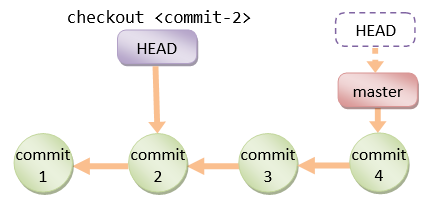
\includegraphics[scale=0.6]{Gambar/gitcheckoutcommit.png}
	\caption{\textit{Checkout} pada \textit{commit}}
	\label{fig:git_checkout}
\end{figure}

\section{JGit}
\label{sec:jgit}
JGit adalah \textit{library} Java murni yang mengimplementasikan Git \textit{version control systems}\cite{JGit}. Dengan menggunakan JGit, operasi-operasi dalam Git bisa dilakukan melalui program Java. Pada subbab berikut dijelaskan beberapa kelas dari \textit{library} JGit. Subbab ini mengacu pada \cite{JGit_java_doc}. 

\subsection{Kelas Repository}
\label{subsec:repository}
Kelas ini merepresentasikan repositori Git. Berikut ini adalah beberapa \textit{method} dalam kelas ini:
\begin{itemize}
\item public void create()\\
Berfungsi untuk membuat repositori Git baru. 
\item public String getBranch()\\
Berfungsi untuk mendapatkan nama \textit{branch} yang ditunjuk oleh \textit{HEAD}.\\
Kembalian: nama dari \textit{branch} yang sedang aktif.
\item public Ref getRef(String name)\\
Berfungsi untuk mendapatkan \textit{reference} berdasarkan nama yang diberikan.\\
Parameter: nama dari \textit{reference}.\\
Kembalian: \textit{object} bertipe Ref.
\end{itemize} 

\subsection{Kelas Ref}
\label{subsec:ref}
Ref di dalam Git merupakan sebuah variabel yang menyimpan ID dari Git Object.
Berikut adalah beberapa \textit{method} yang dimiliki oleh kelas ini:
\begin{itemize}
\item String getName()\\
Berfungsi untuk mengembalikan nama dari suatu Ref.\\
Kembalian: nama dari Ref.
\item ObjectId getObjectId()\\
Berfungsi untuk mengembalikan ID dari suatu Git Object.\\
Kembalian: \textit{object} bertipe ObjectId. Di dalam kelas ObjectId terdapat \textit{method} getName() yang berfungsi untuk mengembalikan ID dari Git Object berupa SHA-1 \textit{hash value}. 
\end{itemize}



\subsection{Kelas FileRepository}
\label{subsec:filerepository}
Kelas ini merupakan turunan dari kelas \textit{Repository}. Berikut ini adalah \textit{construtor} dari kelas ini:
\begin{itemize}
\item public FileRepository(String gitDir) throws IOException\\
\textit{Constructor} ini membuat representasi dari repositori Git. \textit{Constructor} ini melempar IOException jika repositori tidak bisa diakses.\\
Parameter: \textit{path} dari suatu repositori Git.
\end{itemize}

\subsection{Kelas Git}
\label{subsec:Git}
Kelas ini menyediakan API yang mirip Git \textit{command line} untuk berinteraksi dengan repositori Git. Berikut ini adalah \textit{constructor} dan beberapa \textit{method} dalam kelas ini:
\begin{itemize}
\item public Git(Repository repo)\\
\textit{Constructor} ini membuat objek Git yang digunakan untuk berinteraksi dengan repositori Git.\\
Parameter: objek \textit{Repository} yang digunakan untuk berinteraksi. Parameter tidak boleh bernilai \textit{null}. 

\item public static InitCommand init()\\
\textit{Method} ini mengembalikan objek \textit{command} untuk mengeksekusi operasi \textit{init}.\\
Kembalian: objek \textit{InitCommand} yang berfungsi untuk mengumpulkan parameter opsional dan akhirnya mengeksekusi operasi \textit{init}.

\item public AddCommand add()\\
\textit{Method} ini mengembalikan objek \textit{command} untuk mengeksekusi operasi \textit{add}.\\
Kembalian: objek \textit{AddCommand} yang berfungsi untuk mengumpulkan parameter opsional dan akhirnya mengeksekusi operasi \textit{add}.

\item public LogCommand log()\\
\textit{Method} ini mengembalikan objek \textit{command} untuk mengeksekusi operasi \textit{log}.\\
Kembalian: objek \textit{LogCommand} yang berfungsi untuk mengumpulkan parameter opsional dan akhirnya mengeksekusi operasi \textit{log}.



\item public CheckoutCommand checkout()\\
\textit{Method} ini mengembalikan objek \textit{command} untuk mengeksekusi operasi \textit{checkout}.\\
Kembalian: objek \textit{CheckoutCommand} yang berfungsi untuk mengumpulkan parameter opsional dan akhirnya mengeksekusi operasi \textit{checkout}.

\item public CommitCommand commit()\\
\textit{Method} ini mengembalikan objek \textit{command} untuk mengeksekusi operasi \textit{commit}.\\
Kembalian: objek \textit{CommitCommand} yang berfungsi untuk mengumpulkan parameter opsional dan akhirnya mengeksekusi operasi \textit{commit}.

\item public FetchCommand fetch()\\
\textit{Method} ini mengembalikan objek \textit{command} untuk mengeksekusi operasi \textit{fetch}.\\
Kembalian: objek \textit{FetchCommand} yang berfungsi untuk mengumpulkan parameter opsional dan akhirnya mengeksekusi operasi \textit{fetch}.

\item public PushCommand push()\\
\textit{Method} ini mengembalikan objek \textit{command} untuk mengeksekusi operasi \textit{push}.\\
Kembalian: objek \textit{PushCommand} yang berfungsi untuk mengumpulkan parameter opsional dan akhirnya mengeksekusi operasi \textit{push}.

\item public DiffCommand diff()\\
\textit{Method} ini mengembalikan objek \textit{command} untuk mengeksekusi operasi \textit{diff}.\\
Kembalian: objek \textit{DiffCommand} yang berfungsi untuk mengumpulkan parameter opsional dan akhirnya mengeksekusi operasi \textit{diff}.

\item public static CloneCommand cloneRepository()\\
\textit{Method} ini mengembalikan objek \textit{command} untuk mengeksekusi operasi \textit{clone}.\\
Kembalian: objek \textit{CloneCommand} yang berfungsi untuk mengumpulkan parameter opsional dan akhirnya mengeksekusi operasi \textit{clone}.

\item public MergeCommand merge()\\
\textit{Method} ini mengembalikan objek \textit{command} untuk mengeksekusi operasi \textit{merge}.\\
Kembalian: objek \textit{MergeCommand} yang berfungsi untuk mengumpulkan parameter opsional dan akhirnya mengeksekusi operasi \textit{merge}.

\item public PullCommand pull()\\
\textit{Method} ini mengembalikan objek \textit{command} untuk mengeksekusi operasi \textit{pull}.\\
Kembalian: objek \textit{PullCommand}.

\item public CreateBranchCommand branchCreate()\\
\textit{Method} ini mengembalikan objek \textit{command} untuk membuat \textit{branch} baru.\\
Kembalian: objek \textit{CreateBranchCommand}.

\item public ListBranchCommand branchList()\\
\textit{Method} ini mengembalikan objek \textit{command} yang digunakan untuk mengeksekusi operasi \textit{branch}. Operasi ini setara dengan sintaks \texttt{git branch -r/-a}.\\
Kembalian: objek dengan tipe ListBranchCommand.

\item public DeleteBranchCommand branchDelete()\\
\textit{Method} ini mengembalikan objek \textit{command} untuk menghapus \textit{branch}.\\
Kembalian: objek \textit{DeleteBranchCommand}.

\item public ResetCommand reset()\\
\textit{Method} ini mengembalikan objek \textit{command} untuk mengeksekusi operasi \textit{reset}.\\
Kembalian: objek \textit{ResetCommand}.
\end{itemize}

\subsection{Kelas CheckoutCommand}
\label{subsec:checkoutcommand}
Kelas yang digunakan untuk melakukan operasi \textit{checkout}.
Berikut adalah beberapa \textit{method} yang terdapat pada kelas ini:
\begin{itemize}
\item public CheckoutCommand setName(String name)\\
Menentukan nama  \textit{branch} atau \textit{commit} ID untuk melakukan checkout.\\
Parameter: nama dari \textit{branch} atau \textit{commit} ID.\\
Kembalian: \textit{object} CheckoutCommand.
\item public Ref call()\\
Berfungsi untuk menjalankan operasi \textit{checkout}.
\end{itemize}

\subsection{Kelas ListBranchCommand}
\label{subsec:listbranchcommand}
Kelas yang digunakan untuk melakukan operasi \textit{branch} dan mendapatkan daftar \textit{branch}.
Berikut adalah beberapa \textit{method} yang terdapat pada kelas ini:
\begin{itemize}
\item public ListBranchCommand setListMode(ListBranchCommand.ListMode listMode)\\
Menentukan mode yang digunakan untuk mendapatkan \textit{branch}. Jika parameter tidak dimasukkan, hanya daftar \textit{branch} lokal yang didapatkan.\\
Parameter: mode yang digunakan untuk mendapatkan \textit{branch}, parameter ini berupa konstanta.\\
Kembalian: \textit{object} CheckoutCommand.
\item public List<Ref> call()\\
Berfungsi untuk menjalankan operasi \textit{branch}.\\
Kembalian: daftar \textit{branch} dalam bentuk List<Ref>.
\end{itemize}

\subsection{Enum ListBranchCommand.ListMode}
Merupakan sebuah Enum yang berisi mode yang digunakan untuk mendapatkan \textit{branch}.
Berikut ini adalah konstanta yang terdapat pada Enum ini:
\begin{itemize}
\item public static final ListBranchCommand.ListMode ALL\\
Mode ini digunakan untuk mendapatkan semua daftar \textit{branch} baik lokal maupun \textit{remote}. Mode ini setara dengan \textit{option} \texttt{-a} pada sintaks \texttt{git branch -a}.
\item public static final ListBranchCommand.ListMode REMOTE\\
Mode ini digunakan untuk mendapatkan daftar \textit{remote branch}. Mode ini setara dengan \textit{option} \texttt{-r} pada sintaks \texttt{git branch -r}. 
\end{itemize}


\subsection{Kelas LogCommand}
\label{subsec:logcommand}
Kelas yang digunakan untuk melakukan operasi \textit{log}.
Berikut adalah \textit{method} yang terdapat pada kelas ini:
\begin{itemize}
\item public Iterable<RevCommit> call()\\
Berfungsi untuk menjalankan operasi \textit{log}.\\
Kembalian: \textit{commit history} pada \textit{branch} yang sedang aktif. 
\end{itemize}

\subsection{Kelas ResetCommand}
\label{subsec:resetcommand}
Kelas yang digunakan untuk melakukan operasi \textit{reset}.
Berikut adalah beberapa \textit{method} yang terdapat pada kelas ini:
\begin{itemize}
\item public ResetCommand setMode(ResetCommand.ResetType mode)\\
Menentukan tipe \textit{reset}.\\ 
Parameter: tipe \textit{reset}.\\
Kembalian: \textit{object} ResetCommand.
\item public ResetCommand setRef(String ref)\\
Mengatur nama \textit{reference} tujuan dalam operasi \textit{reset}. Secara default, \textit{reference} yang digunakan adalah \textit{HEAD}.\\
Parameter: nama dari \textit{reference}.\\
Kembalian: \textit{object} ResetCommand.
\item public Ref call()\\
Berfungsi untuk menjalankan operasi \textit{reset}.\\
\end{itemize}

\subsection{Kelas ResetCommand.ResetType}
\label{subsec:resettype}
Merupakan \textit{enumeration} yang menentukan tipe \textit{reset} yang digunakan pada operasi \textit{reset}.
\textit{Enumeration} tersebut adalah sebagai berikut:
\begin{itemize}
\item public static final ResetCommand.ResetType SOFT\\
Hanya mengubah posisi \textit{HEAD}. 


\item public static final ResetCommand.ResetType HARD\\
Mengubah posisi \textit{HEAD} ke \textit{reference} tujuan. Selain itu, dilakukan \textit{reset} pada \textit{staging area} dan \textit{working directory} sehingga perubahan yang terdapat pada \textit{staging area} dan \textit{working directory} akan hilang.


\item public static final ResetCommand.ResetType MIXED\\
Mengubah posisi \textit{HEAD} ke \textit{reference} tujuan. Selain itu, dilakukan \textit{reset} pada \textit{staging area} sehingga perubahan yang terdapat pada \textit{staging area} akan dipindahkan ke \textit{working directory}. 
\end{itemize}

\subsection{Kelas RevCommit}
\label{subsec:revcommit}
Kelas ini merupakan \textit{reference} ke \textit{commit} yang ada di \textit{Directed Acyclic Graph}. Berikut ini adalah  beberapa \textit{method} dari kelas ini:
\begin{itemize}
\item public final String getFullMessage()\\
Berfungsi untuk mendapatkan deskripsi dari suatu \textit{commit}.\\
Kembalian: deskripsi dari suatu \textit{commit} dalam bentuk String.

\item public final String getShortMessage()\\
Berfungsi untuk mendapatkan deskripsi dari suatu \textit{commit}. Jika panjang deskripsi \textit{commit} lebih dari satu baris, maka hanya baris pertama yang dikembalikan.\\
Kembalian: baris pertama dari deskripsi \textit{commit} dalam bentuk String.

\item public final String getName()\\
\textit{Method} ini mengembalikan \textit{commit ID}.\\
Kembalian: \textit{commit ID} berupa SHA-1 hash value dalam bentuk String. 

\item public final PersonIdent getAuthorIdent()\\
Berfungsi untuk mendapatkan informasi mengenai \textit{author} yang melakukan \textit{commit}.\\
Kembalian: objek \textit{PersonIdent} yang memuat informasi tentang \textit{author}(nama dan \textit{email}) dan waktu dilakukannya \textit{commit}.
\end{itemize}

\subsection{Kelas PersonIdent}
\label{subsec:personident}
Kelas ini memberikan informasi mengenai \textit{author} dari suatu \textit{commit}. Berikut ini adalah beberapa \textit{method} dari kelas ini:
\begin{itemize}
\item public String getName()\\
Berfungsi untuk mengembalikan nama dari \textit{author} yang melakukan \textit{commit}.\\
Kembalian: nama dari \textit{author}.

\item public String getEmailAddress()\\
Berfungsi untuk mengembalikan alamat \textit{email} dari \textit{author} yang melakukan \textit{commit}.\\
Kembalian: alamat \textit{email} dari \textit{author}.

\item public Date getWhen()\\
Berfungsi mengembalikan waktu dilakukannya suatu \textit{commit} oleh \textit{author}.\\
Kembalian: waktu dilakukannya suatu \textit{commit} berupa objek Date.
\end{itemize}

\section{Selenium WebDriver}
\label{sec:selenium_webdriver}
Selenium adalah seperangkat alat yang secara khusus digunakan untuk mengotomatisasi \textit{web browsers}\cite{Selenium}. Selenium mendukung bahasa pemrograman C\#, Java, Perl, PHP, Python, Ruby, dan JavaScript. Selenium terdiri dari beberapa kakas, yaitu Selenium 1(Selenium RC), Selenium 2(Selenium WebDriver), dan Selenium IDE. Selenium RC merupakan proyek utama \textit{Selenium} untuk waktu yang lama, sebelum akhirnya bergabung dengan WebDriver menjadi Selenium 2. Selenium RC melakukan \textit{automation test} dengan cara menginjeksi kode JavaScript ke \textit{browser}. Selenium RC saat ini sudah \textit{deprecated} dan tidak digunakan lagi. Selenium Webdriver merupakan gabungan dari Selenium RC dan WebDriver. Selenium IDE merupakan \textit{extension} dari \textit{browser} Chrome dan Firefox yang digunakan untuk melakukan \textit{record and playback test} pada \textit{browser}. 
 
WebDriver merupakan kakas untuk mengotomatisasi pengujian pada aplikasi \textit{web}\cite{Selenium_doc}. WebDriver dapat berkomunikasi secara langsung dengan \textit{browser} menggunakan \textit{native support} pada \textit{browser} tanpa melakukan injeksi kode JavaScript. Berikut ini adalah WebDriver yang terdapat pada Selenium WebDriver:
\begin{itemize}
\item ChromeDriver\\
Merupakan implementasi WebDriver yang mengontrol Chrome \textit{browser}.
\item FirefoxDriver\\
Merupakan implementasi WebDriver yang mengontrol Firefox \textit{browser}.
\item OperaDriver\\
Merupakan implementasi WebDriver yang mengontrol Opera \textit{browser}.
\item SafariDriver\\
Merupakan implementasi WebDriver yang mengontrol Safari \textit{browser}.
\item InternetExplorerDriver\\
Merupakan implementasi WebDriver yang mengontrol Internet Explorer \textit{browser}.
\item EdgeDriver\\
Merupakan implementasi WebDriver yang mengontrol Microsoft Edge \textit{browser}.
\end{itemize}

%ChromeDriver merupakan implementasi WebDriver yang mengontrol Chrome \textit{browser}. FirefoxDriver merupakan implementasi WebDriver yang mengontrol Firefox \textit{browser}. OperaDriver merupakan implementasi WebDriver yang mengontrol Opera \textit{browser}. SafariDriver merupakan implementasi WebDriver yang mengontrol Safari \textit{browser}. InternetExplorerDriver merupakan implementasi WebDriver yang mengontrol Internet Explorer \textit{browser}. EdgeDriver merupakan implementasi WebDriver yang mengontrol Microsoft Edge \textit{browser}. HtmlUnitDriver merupakan implementasi WebDriver yang mengontrol HTMLUnit \textit{browser} yang bersifat \textit{headless}(tidak mempunyai GUI). 

Pada skripsi ini \textit{tools} Selenium yang digunakan hanya Selenium WebDriver. Bahasa pemrograman yang digunakan adalah java. WebDriver yang digunakan adalah ChromeDriver. Pemilihan WebDriver ini hanya berdasarkan preferensi penulis saja. Penulis tidak memilih InternetExplorerDriver, EdgeDriver, dan SafariDriver karena InternetExplorerDriver dan EdgeDriver hanya bisa berjalan pada sistem operasi Windows, selain itu SafariDriver hanya bisa berjalan pada sistem operasi macOS. HtmlUnitDriver tidak dipilih karena WebDriver ini tidak mengimplementasikan \textit{interface} untuk mengambil \textit{screenshot}, sehingga tidak bisa dilakukan pengambilan \textit{screenshot}. Pada subbab berikut dijelaskan beberapa kelas dan \textit{interface} dari \textit{library} Selenium WebDriver. Subbab ini mengacu pada \cite{Selenium_java_doc}.

\subsection{Interface WebDriver}
\label{subsec:webdriver}
Merupakan \textit{interface} utama yang digunakan untuk pengujian. Berikut ini adalah beberapa \textit{method} dalam \textit{interface} ini:
\begin{itemize}
\item void close()\\
Berfungsi untuk menutup \textit{window} pada \textit{browser}, jika \textit{window} yang sekarang merupakan satu-satunya \textit{window} yang terbuka maka \textit{browser} akan ditutup.
\item void quit()\\
Berfungsi untuk menutup \textit{browser} dan semua \textit{window} yang sedang terbuka.
\item void get(String url)\\
Berfungsi untuk memuat halaman \textit{web} pada \textit{window} yang sedang aktif. \textit{Method} ini mengirim \textit{HTPP GET Request} untuk memuat halaman, dan \textit{method} ini akan melakukan \textit{blocking} sampai halaman \textit{web} selesai dimuat.\\
Parameter: alamat \textit{url} untuk memuat halaman \textit{web}.
\item String getTitle()\\
Berfungsi untuk mengembalikan judul dari halaman \textit{web} yang sedang aktif.\\
Kembalian: judul dari halaman \textit{web}.
\item String getCurrentUrl()\\
Berfungsi untuk mendapatkan URL yang sedang aktif di \textit{browser}.\\
Kembalian: URL dari halaman \textit{web} yang sedang dimuat di \textit{browser}.

\item WebDriver.Options manage()\\
Berfungsi untuk mendapatkan interface WebDriver.Options.\\
Kembalian: interface dengan tipe WebDriver.Options.  
\end{itemize}

%\subsection{WebDriver.Navigation}
%\label{subsec:webdriver_navigation}
%Kelas ini merupakan \textit{nested class} dari WebDriver. Kelas ini mengatur navigasi pada WebDriver. Berikut ini adalah beberapa \textit{method} dalam kelas ini:
%\begin{itemize}
%\item void back()\\
%Berfungsi untuk berpindah ke halaman \textit{web} sebelumnya.
%\item void forward()\\
%Berfungsi untuk bergerak maju satu halaman \textit{web}. 
%\item void refresh()\\
%Berfungsi untuk melakukan \textit{refresh} pada halaman \textit{web}.
%\item void to(String url)\\
%Berfungsi untuk memuat halaman \textit{web} baru pada \textit{window} yang sedang aktif.\\
%Parameter: URL yang akan dimuat.
%\end{itemize}

\subsection{Interface WebDriver.Options}
\textit{Interface} yang digunakan untuk mengatur \textit{browser menu}. Berikut adalah
\textit{method} yang dimiliki oleh \textit{interface} ini:
\begin{itemize}
\item void deleteAllCookies()\\
Berfungsi untuk menghapus semua \textit{cookie} yang terdapat pada \textit{browser}.
\item WebDriver.Window window()\\
Berfungsi untuk mendapatkan \textit{interface} untuk mengatur \textit{browser window}.\\
Kembalian: objek bertipe WebDriver.Window.
\end{itemize}


\subsection{Interface WebDriver.Window}
\label{subsec:webdriveroption}
\textit{Interface} yang digunakan untuk mengatur \textit{window} pada \textit{browser}. Berikut adalah \textit{method} yang dimiliki oleh \textit{interface} ini:
\begin{itemize}
\item void maximize()\\
Berfungsi untuk membuat ukuran \textit{window} pada \textit{browser} menjadi maksimal.
\end{itemize}

%\subsection{WebElement}
%\label{subsec:webelement}  
%Merupakan \textit{interface} yang  merepresentasikan dari elemen HTML. Berikut ini adalah beberapa \textit{method} yang dimiliki \textit{interface} ini:
%\begin{itemize}
%\item void click()\\
%Berfungsi untuk mengklik suatu elemen HTML.
%\item void submit()\\
%Berfungsi untuk mengirimkan elemen \textit{form} ke \textit{remote server}. Fungsi ini akan melempar \textit{NoSuchElementException} jika elemen yang dikirim tidak berada di dalam \textit{form}. 
%\item String getText()\\
%Berfungsi untuk mendapatkan teks pada suatu elemen.\\
%Kembalian: Teks yang \textit{visible} pada elemen.

%\item void clear()\\
%Berfungsi untuk menghapus teks pada elemen yang digunakan untuk memasukkan teks.
%\item WebElement findElement(By by)\\
%Berfungsi untuk mendapatkan \textit{WebElement} pertama menggunakan metode yang diberikan parameter. \textit{Method} ini akan melempar \textit{NoSuchElementException} jika \textit{WebElement} tidak ditemukan.\\
%Kembalian: \textit{WebElement} pertama yang sesuai dengan mekanisme pencarian.\\
%Parameter: mekanisme pencarian, bisa berupa pencarian dengan \textit{ID}, \textit{class}, dll.

%\item List<WebElement> findElements(By by)\\
%Berfungsi untuk mendapatkan semua \textit{WebElement} sesuai dengan mekanisme yang diberikan parameter.\\
%Kembalian: \textit{list} dari \textit{WebElement}, atau \textit{list} kosong jika pencarian tidak ditemukan.\\
%Parameter: mekanisme pencarian, bisa berupa pencarian dengan \textit{ID}, \textit{class}, dll.
%\item void sendKeys(java.lang.CharSequence... keysToSend)\\
%Berfungsi untuk mengirimkan kumpulan karakter/teks ke elemen \textit{input}. \textit{Method} ini akan melempar %\textit{java.lang.IllegalArgumentException} jika parameter keysToSend bernilai \textit{null}.\\
%Parameter: kumpulan karakter/teks yang dikirim ke elemen.

%\item String getAttribute(String name)\\
%Berfungsi untuk mendapatkan nilai dari \textit{attribute} suatu \textit{web element}.\\
%Kembalian: nilai dari \textit{attribute} dari \textit{web element}.
%\end{itemize} 

%\subsection{By}
%\label{subsec:by}
%Kelas ini mendefinisikan mekanisme pencarian \textit{web element}. Berikut adalah beberapa \textit{method} yang %dimiliki oleh kelas ini:
%\begin{itemize}
%\item public static By className(String className)\\
%Mekanisme pencarian berdasarkan nilai atribut class dari \textit{web element}.\\
%Parameter: nama class dari \textit{web element}.\\
%Kembalian: objek By yang sudah menemukan \textit{web element}.
%\item public static By tagName(String tagName)\\
%Mekanisme pencarian berdasarkan \textit{tag name} dari \textit{web element}.\\
%Parameter: \textit{tag name}  dari \textit{web element}.\\
%Kembalian: objek By yang sudah menemukan \textit{web element}.
%\item public static By id(String id) \\
%Mekanisme pencarian berdasarkan nilai atribut ID dari \textit{web element}.\\
%Parameter: ID dari \textit{web element}.\\
%Kembalian: objek By yang sudah menemukan \textit{web element}.
%\end{itemize} 

\subsection{Kelas ChromeDriver}
\label{subsec:chromedriver}
Merupakan implementasi WebDriver yang mengontrol Chrome \textit{browser}. Berikut adalah \textit{constructor} yang terdapat pada kelas ini:
\begin{itemize}
\item public ChromeDriver()\\
\textit{Constructor} ini membuat instans dengan tipe ChromeDriver.
\end{itemize}

\subsection{Kelas FirefoxDriver}
\label{subsec:firefoxdriver}
Merupakan implementasi WebDriver yang mengontrol Firefox \textit{browser}. Berikut adalah \textit{constructor} yang terdapat pada kelas ini:
\begin{itemize}
\item public FirefoxDriver()\\
\textit{Constructor} ini membuat instans dengan tipe FirefoxDriver.
\end{itemize}

\subsection{Kelas OperaDriver}
\label{subsec:operadriver}
Merupakan implementasi WebDriver yang mengontrol Opera \textit{browser}. Berikut adalah \textit{constructor} yang terdapat pada kelas ini:
\begin{itemize}
\item public OperaDriver()\\
\textit{Constructor} ini membuat instans dengan tipe OperaDriver.
\end{itemize}

\subsection{Kelas SafariDriver}
\label{subsec:safaridriver}
Merupakan implementasi WebDriver yang mengontrol Safari \textit{browser}. Berikut adalah \textit{constructor} yang terdapat pada kelas ini:
\begin{itemize}
\item public SafariDriver()\\
\textit{Constructor} ini membuat instans dengan tipe SafariDriver.
\end{itemize}

\subsection{Kelas InternetExplorerDriver}
\label{subsec:internetexplorerdriver}
Merupakan implementasi WebDriver yang mengontrol Internet Explorer \textit{browser}. Berikut adalah \textit{constructor} yang terdapat pada kelas ini:
\begin{itemize}
\item public InternetExplorerDriver()\\
\textit{Constructor} ini membuat instans dengan tipe InternetExplorerDriver.
\end{itemize}

\subsection{Kelas EdgeDriver}
\label{subsec:edgedriver}
Merupakan merupakan implementasi WebDriver yang mengontrol Microsoft Edge \textit{browser}. Berikut adalah \textit{constructor} yang terdapat pada kelas ini:
\begin{itemize}
\item public EdgeDriver()\\
\textit{Constructor} ini membuat instans dengan tipe EdgeDriver.
\end{itemize}


\subsection{Kelas HtmlUnitDriver}
\label{subsec:htmlunitdriver}
Merupakan implementasi WebDriver yang mengontrol HtmlUnit \textit{browser}. Berikut adalah \textit{constructor} yang terdapat pada kelas ini:
\begin{itemize}
\item public HtmlUnitDriver()\\
\textit{Constructor} ini membuat instans dengan tipe HtmlUnitDriver.
\end{itemize}


\subsection{Interface OutputType}
\label{subsec:output_type}
Merupakan \textit{interface} yang menentukan tipe \textit{output} pada \textit{screenshot}. Terdapat tiga konstanta untuk menentukan tipe \textit{output} pada \textit{screenshot}. Konstanta tersebut adalah sebagai berikut:
\begin{itemize}
\item static final OutputType<String> BASE64\\
Berfungsi untuk mendapatkan \textit{screenshot} dalam bentuk \textit{base64 data}.
\item static final OutputType<byte[]> BYTES\\
Berfungsi untuk mendapatkan \textit{screenshot} dalam bentuk \textit{raw bytes}.
\item static final OutputType<java.io.File> FILE\\
Berfungsi untuk mendapatkan \textit{screenshot} dalam bentuk \textit{temprorary file} yang akan dihapus setelah program keluar dari \textit{Java Virtual Machine}.
\end{itemize}

\subsection{Interface TakesScreenshot}
\label{subsec:takes_screenshot}
Merupakan \textit{interface} yang digunakan untuk mengambil \textit{screenshot}. WebDriver yang mengimplementasikan \textit{interface} ini yaitu ChromeDriver, FirefoxDriver, OperaDriver, InternetExplorerDriver, dan  EdgeDriver. HtmlUnitDriver tidak mengimplentasikan \textit{interface} ini. Berikut adalah \textit{method} yang terdapat dalam \textit{interface} ini:
\begin{itemize}
\item <X> X getScreenshotAs(OutputType<X> target) throws WebDriverException\\
\textit{Method} ini berfungsi untuk mengambil \textit{screenshot} dan mengembalikan hasilnya.\\
Kembalian: objek hasil \textit{screenshot} \\
Parameter: tipe \textit{output} yang diinginkan(lihat subbab \ref{subsec:output_type}).
\end{itemize}


\section{Apache Commons CLI}
\label{subsec:apache_cli}
\textit{Library} Apache Commons CLI menyediakan API untuk melakukan \textit{parsing} argumen \textit{command line} yang dikirimkan ke program\cite{Apache_Commons_CLI}. Apache Commons CLI termasuk ke dalam salah satu \textit{project} Apache Commons. Tujuan utama dari \textit{project} Apache Commons adalah membuat dan melakukan \textit{maintain} pada komponen Java yang \textit{reusable}. Pada subbab berikut dijelaskan beberapa kelas dan \textit{interface} dari \textit{library} Apache Commons CLI. Subbab ini mengacu pada \cite{Apache_java_doc}.

\subsection{Interface CommandLineParser}
\label{subsec:commandlineparser}
Merupakan sebuah \textit{interface}. Kelas yang mengimplementasikan \textit{interface} ini dapat melakukan \textit{parsing} argumen CommandLine berdasarkan pada \textit{option} yang telah ditentukan. Kelas-kelas yang mengimplementasikan \textit{interface} ini yaitu BasicParser, GnuParser, PosixParser, dan DefaultParser. Kelas BasicParser, GnuParser, dan PosixParser sudah \textit{deprecated}. Berikut ini adalah beberapa \textit{method} yang dimiliki \textit{interface} ini: 
\begin{itemize}
\item CommandLine parse(Options options, String[] arguments) throws ParseException\\
Berfungsi untuk melakukan \textit{parsing} argumen \textit{command line} berdasarkan pada \textit{option} yang telah ditentukan. \textit{Method} ini melempar ParseException jika terjadi masalah saat melakukan \textit{parsing}.\\
Parameter: \textit{option} yang telah ditentukan, argumen \textit{command line}.\\
Kembalian: objek CommandLine.

\item CommandLine parse(Options options, String[] arguments,boolean stopAtNonOption) throws ParseException\\
Berfungsi untuk melakukan \textit{parsing} argumen \textit{command line} berdasarkan pada \textit{option} yang telah ditentukan.\\
Parameter: \textit{option} yang telah ditentukan, argumen \textit{command line}, dan suatu \textit{boolean} yang menentukan apakah \textit{parsing} dihentikan jika terdapat \textit{option} yang tidak valid. Jika bernilai \textit{true}, \textit{parsing} akan dihentikan dan semua argumen yang sudah diuraikan akan ditambahkan ke objek CommandLine. Jika bernilai \textit{false}, akan dilempar ParseException bila terdapat \textit{option} yang tidak valid.\\
Kembalian: objek CommandLine.
\end{itemize}


\subsection{Kelas DefaultParser}
\label{subsec:defaultparser}
Merupakan kelas yang mengimplementasikan \textit{interface} CommandLineParser. Berikut adalah \textit{method} yang dimiliki kelas ini:
\begin{itemize}
\item CommandLine parse(Options options, String[] arguments) throws ParseException\\
Berfungsi untuk melakukan \textit{parsing} argumen \textit{command line} berdasarkan pada \textit{option} yang telah ditentukan. \textit{Method} ini melempar ParseException jika terjadi masalah saat melakukan \textit{parsing}.\\
Parameter: \textit{option} yang telah ditentukan, argumen \textit{command line}.\\
Kembalian: objek CommandLine.

\item CommandLine parse(Options options, String[] arguments,boolean stopAtNonOption) throws ParseException\\
Berfungsi untuk melakukan \textit{parsing} argumen \textit{command line} berdasarkan pada \textit{option} yang telah ditentukan.\\
Parameter: \textit{option} yang telah ditentukan, argumen \textit{command line}, dan suatu \textit{boolean} yang menentukan apakah \textit{parsing} dihentikan jika terdapat \textit{option} yang tidak valid. Jika bernilai \textit{true}, \textit{parsing} akan dihentikan dan semua argumen yang sudah diuraikan akan ditambahkan ke objek CommandLine. Jika bernilai \textit{false}, akan dilempar ParseException bila terdapat \textit{option} yang tidak valid.\\
Kembalian: objek CommandLine.
\end{itemize}

\subsection{Kelas CommandLine}
\label{subsec:commandline}
Kelas ini merepresentasikan kumpulan \textit{option} hasil \textit{parsing}.
Berikut ini adalah beberapa \textit{method} yang dimiliki kelas ini: 
\begin{itemize}
\item public String getOptionValue(String opt)\\
Berfungsi untuk mendapatkan nilai dari suatu \textit{option} sesuai dengan namanya.\\
Parameter: nama dari \textit{option}.\\
Kembalian: nilai dari suatu \textit{option}. Jika \textit{option} tidak ditemukan, akan mengembalikan \textit{null}.
\item public String[] getOptionValues(Option option)\\
Berfungsi untuk mendapatkan kumpulan nilai dari suatu \textit{option}.
Parameter: nama dari \textit{option}.\\
Kembalian: kumpulan nilai dari suatu \textit{option} dengan tipe \textit{array of String}. Jika \textit{option} tidak ditemukan, akan mengembalikan \textit{null}.
\item public Option[] getOptions()\\
Berfungsi untuk mengembalikan \textit{option} hasil \textit{parsing}.\\ 
Kembalian: \textit{array} dari \textit{option} hasil \textit{parsing}.


\end{itemize}

\subsection{Kelas Options}
\label{subsec:options}
Kelas ini merepresentasikan kumpulan dari objek Option. Berikut ini adalah \textit{method} yang dimiliki kelas ini: 
\begin{itemize}
\item public Options addOption(Option opt)\\
Berfungsi untuk menambahkan \textit{option}.\\
Parameter: \textit{option} yang akan ditambahkan.\\
Kembalian: hasil dari \textit{option} yang ditambahkan.

\end{itemize}


\subsection{Kelas Option}
\label{subsec:option}
Kelas ini merepresentasikan sebuah Command Line Option. Berikut ini adalah beberapa \textit{method} yang dimiliki kelas ini: 
\begin{itemize}
\item public String getLongOpt()\\
Berfungsi untuk mendapatkan nama panjang dari suatu \textit{option}.\\
Kembalian: nama panjang dari suatu \textit{option}.
\item public String getValue()\\
Berfungsi untuk mendapatkan nilai dari \textit{option}.\\
Kembalian: nilai dari \textit{option}. Jika terdapat lebih dari satu kembalian, hanya nilai pertama yang dikembalikan. Jika tidak ada nilai, akan mengembalikan \textit{null}.

\item public String[] getValues()\\
Berfungsi untuk mendapatkan nilai-nilai dari \textit{option}.\\
Kembalian: nilai-nilai dari \textit{option} berupa \textit{array of String}. Jika tidak ada nilai, akan mengembalikan \textit{null}.

\item public boolean hasArg()\\
Berfungsi untuk mengetahui apakah suatu \textit{option} membutuhkan argumen.\\
Kembalian: \textit{true} jika \textit{option} ini membutuhkan argumen , \textit{false} jika \textit{option} ini tidak membutuhkan argumen.

\item public boolean hasArg()\\
Berfungsi untuk mengetahui apakah suatu \textit{option} dapat menerima lebih dari satu argumen.\\
Kembalian: \textit{true} jika \textit{option} ini dapat menerima lebih dari satu argumen , \textit{false} jika tidak.

\item public String getDescription()\\
Berfungsi untuk mendapatkan deskripsi dari suatu \textit{option}.\\
Kembalian: deskripsi dari \textit{option} ini.
\item public String getArgName()\\
Berfungsi untuk mendapatkan nama dari suatu \textit{option}.\\
Kembalian: nama dari argumen suatu \textit{option}


\end{itemize}

\subsection{Kelas Option.Builder}
\label{subsec:optionbuilder}
Kelas ini merupakan \textit{nested class} dari kelas Option. Kelas ini digunakan untuk membuat objek Option berdasarkan parameter yang diberikan. Berikut ini adalah beberapa \textit{method} yang dimiliki kelas ini: 
\begin{itemize}
\item public Option.Builder desc(String description)\\
Berfungsi untuk memberikan deskripsi pada \textit{option}.\\
Parameter: deskripsi dari \textit{option}.\\
Kembalian: objek Option.Builder yang bisa digunakan untuk \textit{method chaining}.

\item public Option.Builder longOpt(String longOpt)\\
Berfungsi untuk memberikan nama panjang pada \textit{option}.\\
Parameter: nama panjang \textit{option}.\\
Kembalian: objek Option.Builder yang bisa digunakan untuk \textit{method chaining}.

\item public public Option.Builder hasArg()\\
Berfungsi untuk menyatakan bahwa \textit{option} ini membutuhkan argumen.\\
Kembalian: objek Option.Builder yang bisa digunakan untuk \textit{method chaining}.

\item public public Option.Builder hasArgs()\\
Berfungsi untuk menyatakan bahwa \textit{option} ini membutuhkan argumen dimana jumlah argumen bisa lebih dari satu.\\
Kembalian: objek Option.Builder yang bisa digunakan untuk \textit{method chaining}.

\item public Option.Builder argName(String argName)\\
Berfungsi untuk memberi nama pada argumen.\\
Parameter: nama argumen.\\
Kembalian: objek Option.Builder yang bisa digunakan untuk \textit{method chaining}.

\item public Option.Builder required(boolean required)\\
Berfungsi untuk menyatakan bahwa \textit{option} ini wajib ada.\\
Parameter: variabel bertipe \textit{boolean} yang menentukan apakah \textit{option} ini wajib ada.\\
Kembalian: objek Option.Builder yang bisa digunakan untuk \textit{method chaining}.

\item public Option build()\\
Berfungi untuk membuat objek Option berdasarkan nilai pada kelas Option.Builder.\\
Kembalian: objek Option.

\end{itemize}


